	% This text is proprietary.
% It's a part of presentation made by myself.
% It may not used commercial.
% The noncommercial use such as private and study is free
% Sep. 2005 
% Author: Sascha Frank 
% University Freiburg 
% www.informatik.uni-freiburg.de/~frank/

% \documentclass[handout]{beamer}
% % Impression 4p / feuille
% \usepackage{pgfpages}
% \pgfpagesuselayout{4 on 1}[border shrink=1mm]


%\documentclass[aspectratio=169]{beamer}
\documentclass{beamer}

\usepackage{lmodern}
\usepackage{tikz}
\usepackage{subfig}
\usetikzlibrary{shapes}
\usetheme{Boadilla}


\usepackage{color,xcolor}
\usepackage{appendixnumberbeamer}
\usepackage{media9}
\usepackage[export]{adjustbox}
%\usepackage[dvipsnames]{xcolor}
\newcommand*{\mathcolor}{}
\def\mathcolor#1#{\mathcoloraux{#1}}
\newcommand*{\mathcoloraux}[3]{%
  \protect\leavevmode
  \begingroup
    \color#1{#2}#3%
  \endgroup
}

\newcommand\Wider[2][3em]{%
\makebox[\linewidth][c]{%
  \begin{minipage}{\dimexpr\textwidth+#1\relax}
  \raggedright#2
  \end{minipage}%
  }%
}

\newcommand{\dr}{\mathop{\mathrm{d}r}}
\newcommand{\dth}{\mathop{\mathrm{d}\theta}}
\newcommand{\diag}{\mathop{\mathrm{diag}}}





\newcommand{\dz}{\mathop{\mathrm{d}z}}
\newcommand{\dx}{\mathop{\mathrm{d}x}}
\newcommand{\dy}{\mathop{\mathrm{d}y}}
\newcommand{\ds}{\mathop{\mathrm{d}s}}
\newcommand{\dOmega}{\mathop{\mathrm{d}\Omega}}
\newcommand{\diff}[1]{\mathop{\mathrm{d}{#1}}}

\usepackage{amsmath}
\usepackage{tabularx}
\usepackage{booktabs}
\usepackage{colortbl}
\usetikzlibrary{calc}
\pgfdeclarelayer{background}
\pgfdeclarelayer{foreground}
\pgfsetlayers{background,main,foreground}
%\setbeamertemplate{background canvas}[vertical shading]%
%  [top=blue!1,bottom=blue!30]
\setbeamertemplate{navigation symbols}{}
\newcommand*\up{\textcolor{green}{%
  \ensuremath{\blacktriangle}}}
\newcommand*\down{\textcolor{red}{%
  \ensuremath{\blacktriangledown}}}
\newcommand*\const{\textcolor{darkgray}%
  {\textbf{--}}}

\usepackage[style=authoryear]{biblatex}


\usepackage{xcolor}


% tikz stuff
\usepackage{tikz}
\usetikzlibrary{shapes,arrows}
\usetikzlibrary{positioning}
\usepackage{pgfplots}
\pgfplotsset{compat=newest}
\tikzset{%
    block/.style    = {draw, thick, rectangle, minimum height = 3em,
        minimum width = 6em},
    gain/.style     = {draw, thick, isosceles triangle, minimum height = 2em,
        isosceles triangle apex angle=60},
    port/.style     = {inner sep=0pt, font=\tiny},
    sum/.style n args = {4}{draw, circle, node distance = 2cm, minimum size=5mm, alias=sum,
        append after command={
            node at (sum.north) [port, below=1pt] {$#1$}
            node at (sum.west) [port, right=1pt] {$#2$}
            node at (sum.south) [port, above=1pt] {$#3$}
            node at (sum.east) [port, left=1pt] {$#4$}
        },
    }, % Adder
    joint/.style    = {circle, draw, fill, inner sep=0pt, minimum size=2pt},
    input/.style    = {coordinate}, % Input
    output/.style   = {coordinate} % Output
}



\newcommand{\highlight}[1]{%
  \colorbox{red!50}{$\displaystyle#1$}}

\addbibresource{references.bib}
%% movie
\newcommand{\citeref}[1]{{\tiny#1}}
\newcommand{\colorinter}[1]{{\color{red}#1}}
\newcommand{\norm}[1]{\left\lVert#1\right\rVert} 
\newcommand*\Laplace{\mathop{}\!\mathbin\Delta}
%\newcommand*\gradient{\mathop{}\!\mathbin{\vec{\nabla}}}
\newcommand*\gradient{\mathop{}\!\mathbin{\vec{grad}}}
%\newcommand*{\divergence}{\mathop{}\!\mathbin{{\vec{\nabla} \cdot}}}
\newcommand*{\divergence}{\mathop{}\!\mathbin{{div}}}


% numbering...
\setbeamercolor{mycolor}{fg=white,bg=blue}

\defbeamertemplate*{footline}{shadow theme}{%
\leavevmode%
\hbox{\begin{beamercolorbox}[wd=.3\paperwidth,ht=2.5ex,dp=1.125ex,leftskip=.3cm plus1fil,rightskip=.3cm]{author in head/foot}%
    \usebeamerfont{author in head/foot}\hfill\insertshortauthor
\end{beamercolorbox}%
\begin{beamercolorbox}[wd=.6\paperwidth,ht=2.5ex,dp=1.125ex,leftskip=.3cm,rightskip=.3cm plus1fil]{title in head/foot}%
    \usebeamerfont{title in head/foot}\insertshorttitle\hfill%
\end{beamercolorbox}%
\begin{beamercolorbox}[wd=.1\paperwidth,ht=2.5ex,dp=1.125ex,leftskip=.3cm,rightskip=.3cm plus1fil]{mycolor}%
\hfill\insertframenumber\,/\,\inserttotalframenumber
\end{beamercolorbox}}%
\vskip0pt%
}
% end numbering

\AtBeginSection[] {
  \begin{frame}[plain]
    \frametitle{Overview}
    \tableofcontents[currentsection]
  \end{frame}
  \addtocounter{framenumber}{-1}
}

\usepackage{attachfile2}
\newcommand{\includemovie}[2][]{
    \includemedia[
        #1,
        activate=pageopen, transparent,
        addresource=figures/#2.mp4,%addresource=figures/#2.png,
        flashvars={
            source=figures/#2.mp4%&image=figures/#2.png&
            stretching=uniform&start=1&
            screencolor=white& %improves render in light  backgrounds
            controlbar.position=over&controlbar.idlehide=true&
            autostart=true&repeat=always&smoothing=true
            %&bufferlength=10 % may improve repetition of short videos
        }
    ]{ % for disabled content (in most cases this is fallback)
        \begin{tabular}{ll}
            \mbox{
               %\href{run:figures/#2.mp4} % for not embedded fallback
                \textattachfile[color={0 0 0}]{figures/#2.mp4} % for embedded fallback
                {\texttt{|\kern-.23em>}} % poor play button
            } & \raisebox{-\height}{\includegraphics[#1]{figures/#2}}
        \end{tabular}
    }{player.swf}
}

\begin{document}
\title[Port-Hamiltonian modeling, discretization and feedback control of a circular water tank]{PH modeling, discretization and feedback control of a circular water tank}
\author[Fl\'{a}vio Luiz Cardoso-Ribeiro]{Fl\'{a}vio Luiz Cardoso-Ribeiro}



\titlegraphic{
	
\includegraphics[width=2cm]{figures/logoITA}\hspace*{1.cm}~
	
\includegraphics[width=2cm]{figures/logoISAE}
   
}

\date{December 13th 2019}



%\frame{\titlepage}  
\frame{
\begin{center}
	IEEE Conference on Decision and Control (CDC 2019)
\end{center}
\vspace{1cm}
\begin{center}
 { \Large \textbf{Port-Hamiltonian modeling, discretization and feedback control of a circular water tank}}
 \end{center}

\begin{center}
 {\scriptsize Fl\'avio L. CARDOSO-RIBEIRO$^1$, Andrea BRUGNOLI$^2$, Denis MATIGNON$^2$, Laurent LEF\`EVRE$^3$}
\\
\vspace{1cm}
 {\tiny
 $^1$Instituto Tecnologico de Aeronautica, ITA, Brazil\\
 $^2$Univ. de Toulouse, ISAE-SUPAERO, France\\
 $^3$Univ. Grenoble Alpes, LCIS, France
 }
\end{center} 

\begin{center}
  \begin{minipage}{2.5cm}
    \centering
    
\includegraphics[height=1.cm]{figures/logoITA}
    \end{minipage}
   %\begin{minipage}{2.3cm}
    %\centering
    %
\includegraphics[height=1.cm]{figures/logoCAPES}
    %\end{minipage}
  \begin{minipage}{2.3cm}
    \centering
    
\includegraphics[height=1.cm]{figures/logoISAE}
    \end{minipage}
    \begin{minipage}{2.3cm}
      \centering
      
\includegraphics[height=1.cm]{figures/logoLCIS}
    \end{minipage}
  \end{center}

\begin{center}
Nice, France, 13th December 2019.
\end{center}


}  

\section{Introduction}
\frame{\frametitle{Applications for using Shallow Water Equations and sloshing problems}

\begin{minipage}{0.48\textwidth}
  %\hspace{-5cm}
  \centering
	\includemedia[
  addresource = figures/Tsunami.mp4,
  activate=pageopen,
  width=6cm,height=3cm,
  width=0.5\paperwidth,
  flashvars={source=figures/Tsunami.mp4
            &loop=true}
  ]{}{VPlayer.swf}

  \small
  Ocean waves propagation
\end{minipage}
\begin{minipage}{0.48\textwidth}
  \centering
  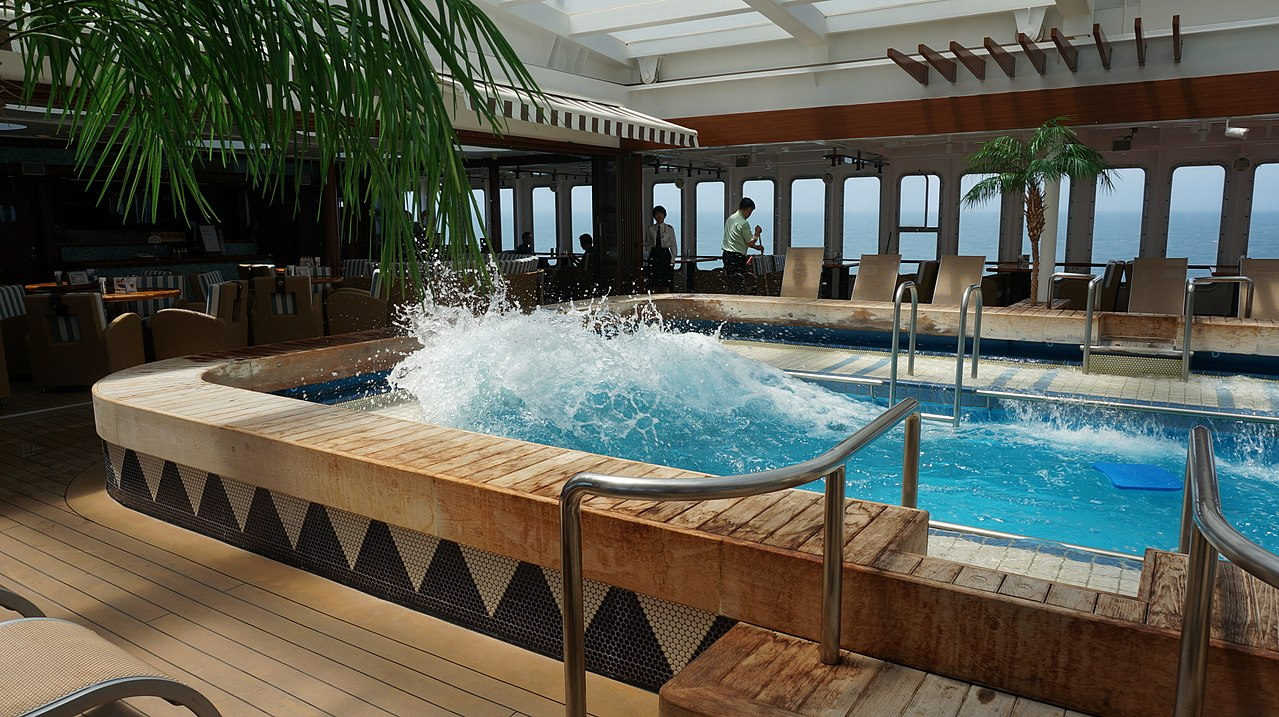
\includegraphics[width=0.9\linewidth]{figures/sloshpool.jpg}
  
  \small
  Waves in a swimming pool.
\end{minipage}


\pause
\begin{minipage}{0.48\textwidth}
  \centering
  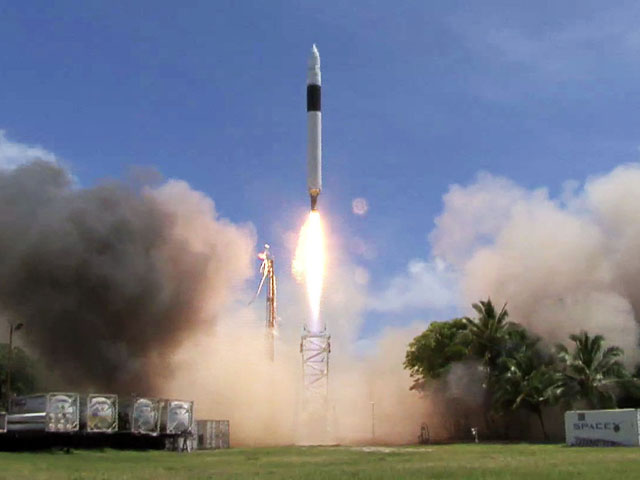
\includegraphics[width=0.7\linewidth]{figures/falcon1.jpg}

  \small Falcon 1 rocket with liquid propellant
\end{minipage}
\begin{minipage}{0.48\textwidth}
  \centering
  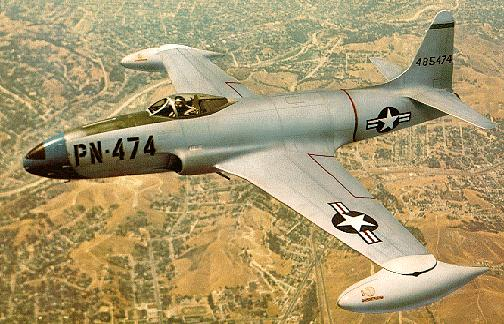
\includegraphics[width=0.8\linewidth]{figures/f80.jpg}
  
  \small
  F80 airplane with tip tanks
\end{minipage}

}

\frame{\frametitle{Examples of circular water tanks for research of wave dynamics and control}

\small
\begin{minipage}{0.48\textwidth}
  \centering
  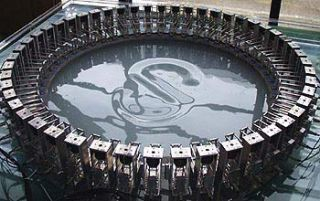
\includegraphics[width=0.8\linewidth]{figures/amoeba.jpg}

  Advanced Multiple Organized Experimental BAsin (AMOEBA)
\end{minipage}
\begin{minipage}{0.48\textwidth}
  \centering
  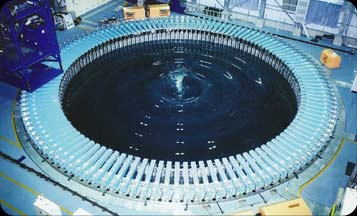
\includegraphics[width=0.8\linewidth]{figures/NMRIdeepseabasin.jpeg}
  
  Deep sea experiment - National Maritime Research Institute - Japan
\end{minipage}

\centering
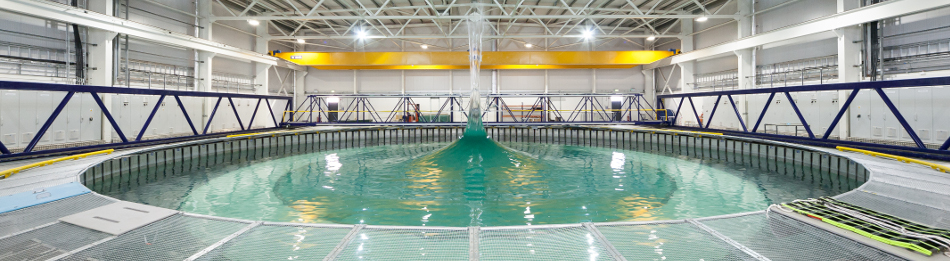
\includegraphics[width=0.8\linewidth]{figures/flowave.jpeg}

FloWave - University of Edingburgh

}

\frame{\frametitle{Port-Hamiltonian modeling, discretization and control}


\begin{minipage}{0.46\textwidth}
	\begin{block}{Infinite-dimensional pHs}
	 \small
		% \begin{equation}
			% \nonumber
			% \begin{split}
				% \dot{\pmb{x}}(z,t) & = \mathcal{J} \delta_{\pmb{x}} H\left(\pmb{x}(z,t)\right) \,,
			% \end{split}
		 % \end{equation}
		 % With boundary conditions:
		 % \begin{equation}
			% \nonumber
			% \begin{split}
				% {\pmb{u}_\partial} = \mathcal{B} \pmb{x} \,,\quad {\pmb{y}_\partial} = \mathcal{C} \pmb{x}
			% \end{split}
		 % \end{equation}
		% And the power balance: $\mathcolor{red}{\dot{H} = \pmb{y}_{\partial}^T \pmb{u}_{\partial}}$.
		\begin{equation}
			\nonumber
				\dot{\pmb{x}}(z,t)  = \mathcal{J} \pmb{e}(z,t)\,, 
     \end{equation}
     where $z \in \Omega$:
     
     $\pmb{x}(z,t)$ is the vector of energy variables;

     $\pmb{e}(z,t) := \delta_{\pmb{x}} H(\pmb{x})$ is the vector of co-energy variables.

		 With boundary control \& observation:
		 \begin{equation}
			\nonumber
			\begin{split}
				\mathcolor{blue}{{u}_\partial} = \mathcal{B} \pmb{e} \,,\quad \mathcolor{blue}{{y}_\partial} = \mathcal{C} \pmb{e}
			\end{split}
		 \end{equation}
		 \vspace{-0.6cm}
		 
		\textbf{Power-balance}:

		$\dot{H} = <\mathcolor{blue}{{y}_{\partial},{u}_{\partial}}>_{\partial \Omega}$
	\end{block}
\end{minipage}
\begin{minipage}{0.05\textwidth}
    \scriptsize	\centering		
    \pause
			$\ \Longrightarrow$
\end{minipage}
\begin{minipage}{0.44\textwidth}
	\begin{exampleblock}{Finite-dimensional approximation:}
	  \small
		  \begin{equation}
		 \nonumber
			\begin{split}
				\dot{\pmb{x}}(t) & = J \pmb{e}(t) + B_\partial \mathcolor{blue}{\pmb{u}_\partial} \,, \\
				\mathcolor{blue}{\pmb{y}_\partial} &= B^T\pmb{e}(t)  +  D_\partial \pmb{u}_\partial \,,
			\end{split}
		 \end{equation}
		 \vspace{-0.2cm}
		 		 
     where:
     
     $\pmb{x}(t)\in \mathbb{R}^N$ is the vector of energy variables;

     $\pmb{e}(t)= \nabla_{\pmb{x}} H_d(\pmb{x}) \in \mathbb{R}^N$ is the vector of co-energy variables;

     \textbf{Power-balance:}
		 
		 $\dot{H}_d = \mathcolor{blue}{\pmb{y}_\partial^T\pmb{u}_\partial}$.
	\end{exampleblock}
\end{minipage}
\pause
\begin{alertblock}{Output feedback control: u = -k y}
  \centering $\dot{H}  = - y^T k y  \leq 0 $\,.
\end{alertblock}

}


\frame{\frametitle{Goals of this contribution}

\begin{enumerate}
  \item Present the 2D Shallow Water Equations as a port-Hamiltonian system in polar coordinates; \pause
  \item Assuming revolution symmetry of boundary and initial conditions, reduce to 1D; \pause
  \item Perform power-preserving semi-discretization to both 1D and 2D systems using the Partitioned Finite Element Method\onslide<3->{\footnotemark.} \pause
  \item Use of output feedback to stabilize the plant.
\end{enumerate}

\footnotetext[1]{\footnotesize \onslide<3->{CARDOSO-RIBEIRO, F.L., MATIGNON, D., LEF\`EVRE, L., ``A structure-preserving Partitioned Finite Element Method for the 2D wave equation'', IFAC LHMNLC (2018)}}
}


\section{Modeling}

\frame{\frametitle{Modeling: The Shallow Water Equations in polar coordinates as port-Hamiltonian Systems (1/2)}


  Let us consider the disc $\Omega=D_R$ of radius $R>0$ with boundary $\partial \Omega=C_R$, the circle of radius $R$. Polar coordinates: $r$, $\theta$.

\pause
\begin{exampleblock}{The total energy is given by:}
  \centering
$E = \frac{1}{2}\int_{D_R} [\rho g h^2 + \rho h((u^r)^2+(u^{\theta})^2)]  \, r\,\dr\dth\,.$

\end{exampleblock}
\pause

\begin{block}{Energy variables are:}
\begin{itemize}
    \item the fluid height $\alpha_q := h(t,r,\theta)$,
    \item the fluid linear momentum given by the vector  $\pmb{{\alpha}_p}:=\rho\,[u^r(t,r,\theta),u^{\theta}(t,r,\theta)]^T$.
\end{itemize}
\end{block}
\pause
\begin{alertblock}{The Hamiltonian is given by:}
  \centering
$H = \int_{D_R} [\frac{1}{2}\rho g \alpha_q^2 + \frac{1}{2\rho}  \alpha_q |\pmb{{\alpha}_p}|^2]\,  r\,\dr\dth\,.$
\end{alertblock}
}

\frame{\frametitle{Modeling: The Shallow Water Equations in polar coordinates as port-Hamiltonian Systems (2/2)}

\begin{columns}
  \begin{column}{0.46\textwidth}
  \begin{exampleblock}{The 2D SWE equations:}
    \small
    \begin{equation}
      \nonumber
      \left[ \begin{array}{c} \dot{\alpha_q} \\ \pmb{\dot{\alpha}_p}  \end{array} \right]  = \left[ \begin{array}{cc} 0 & - \mbox{div} \\ -\pmb{grad} & 0 \end{array} \right] \left[ \begin{array}{c}  e_q \\ \pmb{e_p} \end{array} \right]\,,
    \end{equation}    
  {\tiny where:\vspace{-0.2cm}
  \begin{equation}
    \nonumber
    \begin{split}
    \mbox{div}\left[ \begin{matrix} A_r \\ A_\theta \end{matrix} \right] & := \frac{1}{r}\frac{\partial(r A_r)}{\partial r} + \frac{1}{r}\frac{\partial A_\theta}{\partial \theta}\,,\\
    \pmb{grad}(f) & := \left[\begin{matrix} \frac{\partial f}{\partial r}  \\  \frac{1}{r}\frac{\partial f}{\partial \theta} \end{matrix}\right] \,.
    \end{split}\vspace{-0.3cm}
  \end{equation}}
  \end{exampleblock}
  \end{column}
  \pause
  \begin{column}{0.52\textwidth}
    \begin{block}{Hamiltonian and co-energy}
      \small
  \begin{equation}
    \nonumber
    H = \int_{D_R} [\frac{1}{2}\rho g \alpha_q^2 + \frac{1}{2\rho}  \alpha_q |\pmb{{\alpha}_p}|^2]\,  r\,\dr\dth\,.
  \end{equation}
  {\tiny
  and the co-energy variables are computed as:
  \begin{equation}
    \nonumber
    \begin{split}
    e_q :=& \delta_q H=\rho g \alpha_q +\frac{1}{2\rho}|\pmb{{\alpha}_p}|^2 = \text{\color{red} total pressure}\,,\\
    \pmb{e_p} :=& \delta_{\pmb{p}} H=\frac{1}{\rho}  \alpha_q \pmb{{\alpha}_p} =h\,[u^r(t,r,\theta), u^{\theta}(t,r,\theta)]^T = \text{\color{red} vol. flow}\,.
    \end{split}
  \end{equation}}
  \end{block}
  \end{column}
  \end{columns}
  \pause
  \begin{alertblock}{Power balance}
    \small    
    \begin{equation}
      \nonumber
      \frac{d}{dt} H = \int_{D_R} [\dot{\alpha}_q e_q + \pmb{\dot{\alpha}_p} \cdot \pmb{{e}_p} ] \, r\,\dr\dth\,,
      = \int_{C_R} u_{\partial}(\theta,t)\,y_{\partial}(\theta,t)\,R\,\dth\,.
    \end{equation}
  {\tiny where the boundary input is:$  u_{\partial}(\theta,t):= - \pmb{e_p} \cdot \pmb{n}= - e_p^r(R, \theta, t) = \text{\color{red}boundary ingoing volumetric fluid flux}\,,$
  
  and its power-conjugated boundary output is given by:
  $    y_\partial (\theta,t) := e_q(R, \theta,t)\, = \text{\color{red} boundary pressure}.$}
  \end{alertblock}
  


}

\frame{\frametitle{Modeling: Reduction to 1D by symmetry (1/2)}

\begin{block}{Energy/Hamiltonian of the 1D system:}
In the symmetric case, $u^\theta = 0$. Furthermore, the energy and co-energy variables are constant in $\theta$. Thus, the Hamiltonian simplifies as:
\begin{eqnarray}
  \nonumber
	H=  \frac{1}{2}\int_{D_R} [\rho g h^2 + \rho h((u^r)^2+(u^{\theta})^2)]  \, r\,\dr\dth\,. = 2 \pi \bar{H}\,,
\end{eqnarray}
where:
\begin{equation}
  \nonumber
	\bar{H} = \frac{1}{2}\int_{r=0}^R [\rho g h^2 + \rho h(u^r)^2]  \, r\,\dr\,.
\end{equation}
\end{block}
\pause
\begin{exampleblock}{The equations of motion also simplifies  as:}
\begin{equation}
	\nonumber
	\left[ \begin{array}{c} \dot{h} \\  \rho \dot{u}^r \end{array} \right]  = \underbrace{\left[ \begin{array}{cc} 0 & - \frac{1}{r}\frac{\partial }{\partial r}\left( r \,. \right) \\ -\frac{\partial}{\partial r}\left(  . \right) & 0 \end{array} \right]}_{\cal J}\left[ \begin{array}{c}  \rho g h + \frac{1}{2}\rho (u^r)^2  \\ h u^r \end{array} \right]\,.
\end{equation}
\end{exampleblock}

}



\frame{\frametitle{Modeling: Reduction to 1D by symmetry (2/2)}
\begin{columns}
  \begin{column}{0.46\textwidth}
  \begin{exampleblock}{The 1D reduced equations:}
    \small
    Using the fluid height $\alpha_q = h(t,r)$ and the radial linear momentum $\alpha_p = \rho u^r(t,r)$ as energy variables, we get:
    {\scriptsize
    \begin{equation}
      \nonumber
    \left[ \begin{array}{c} \dot{\alpha_q} \\  \dot{\alpha}_p \end{array} \right]  = \underbrace{ \left[ \begin{array}{cc} 0 & - \frac{1}{r}\frac{\partial }{\partial r}\left( r \,. \right) \\ -\frac{\partial}{\partial r}\left(  . \right) & 0 \end{array} \right]}_{\mathcal{J}} \left[ \begin{array}{c}  e_q \\ e_p \end{array} \right]
    \end{equation}}
  \end{exampleblock}
  \end{column}
  \pause
  \begin{column}{0.52\textwidth}
    \begin{block}{Hamiltonian and co-energy}
      \small
      \begin{equation}
        \nonumber
        \bar{H} = \frac{1}{2}\int_{r=0}^R [\rho g \alpha_q^2 + \frac{1}{\rho} \alpha_q \alpha_p^2]  \, r\,\dr\,,
      \end{equation}
  {\tiny
  and the co-energy variables are computed as:
  \begin{equation}
    \nonumber
    \begin{split}
    e_q &= \frac{\delta \bar{H}}{\delta \alpha_q} = \rho g \alpha_q + \frac{\alpha_p^2}{2\rho} = \text{\color{red} pressure}\,,\\
    e_p & = \frac{\delta \bar{H}}{\delta \alpha_p} = \frac{\alpha_q \alpha_p}{\rho} = \text{\color{red} volumetric radial flow}\,.
    \end{split}
  \end{equation}}
  \end{block}
  \end{column}
  \end{columns}
  \pause
  \begin{alertblock}{Power balance}
    \small    
    \begin{equation}
      \nonumber
      \begin{split}
        \frac{d}{dt} \bar{H} &= \int_{r=0}^{R}{(\dot{\alpha}_q e_q + \dot{\alpha}_p e_p) r \dr} \,,\\
        &= - R \,e_p(t,R) \,e_q(t,R)\,.
      \end{split}
    \end{equation}
  \end{alertblock}
  


}

\section{Power-preserving semi-discretization}
\frame{\frametitle{The partitioned weak-form (1/2)}
\begin{columns}
\begin{column}{0.49\textwidth}
  \begin{block}{The 2D SWE:}
    \begin{equation}
      \nonumber
      \left[ \begin{array}{c} \dot{\alpha_q} \\ \pmb{\dot{\alpha}_p}  \end{array} \right]  = \left[ \begin{array}{cc} 0 & - \mbox{div} \\ -\pmb{grad} & 0 \end{array} \right] \left[ \begin{array}{c}  e_q \\ \pmb{e_p} \end{array} \right]\,
    \end{equation}
  \end{block}
  \end{column}
  \pause
  \begin{column}{0.49\textwidth}
    \begin{exampleblock}{Weak-form:}
      \scriptsize
      Taking arbitrary test functions $v_q$ and $\pmb{v_p}$:
      \vspace{-.3cm}
      \begin{equation}
        \nonumber
        \begin{split}
          \int_{D_R} {v_q {\dot{\alpha}_q}}\,r\, \dr \dth & = - \int_{D_R} {v_q \left( \pmb{\nabla}  \cdot \pmb{e}_{\pmb{p}}  \right)}\,r\, \dr \dth \,,\\
          \int_{D_R}  {\pmb{v_p} \cdot \pmb{\dot{\alpha}_p}}\,r\, \dr \dth & = - \int_{D_R} {\pmb{v_p} \cdot  \pmb{\nabla} e_q}\,r\, \dr \dth \,.
        \end{split}
      \end{equation}      
    \end{exampleblock}
  \end{column}
\end{columns}
  \pause
\begin{alertblock}{Integrating the first equation by parts, we get:}
  \scriptsize
  \vspace{-0.5cm}
  \begin{equation}
    \nonumber
    \begin{split}
      \int_{D_R} {v_q {\dot{\alpha}_q}}\,r\, \dr \dth  =& \int_{D_R} { \left( \pmb{\nabla}v_q \right) \cdot \pmb{e}_{\pmb{p}}}\,r\, \dr \dth - \int_{C_R} v_q \, \pmb{n} \cdot \pmb{e}_{\pmb{p}} \,R\,\dth\,,\\
      \int_{D_R}  {\pmb{v_p} \cdot \pmb{\dot{\alpha}_p}}\,r\, \dr \dth  =& - \int_{D_R} {\pmb{v_p} \cdot  \pmb{\nabla} e_q}\,r\, \dr \dth \,.
    \end{split}
  \end{equation}  
\end{alertblock}
}

\frame{\frametitle{The partitioned weak-form (2/2)}
\begin{alertblock}
  \scriptsize
  \vspace{-0.5cm}
  \scriptsize
  \begin{equation}
    \nonumber
    \begin{split}
      \int_{D_R} {v_q {\dot{\alpha}_q}}\,r\, \dr \dth  =& \int_{D_R} { \left( \pmb{\nabla}v_q \right) \cdot \pmb{e}_{\pmb{p}}}\,r\, \dr \dth - \int_{C_R} v_q \, \underbrace{\pmb{n} \cdot \pmb{e}_{\pmb{p}}}_{-u_\partial} \,R\,\dth\,,\\
      \int_{D_R}  {\pmb{v_p} \cdot \pmb{\dot{\alpha}_p}}\,r\, \dr \dth  =& - \int_{D_R} {\pmb{v_p} \cdot  \pmb{\nabla} e_q}\,r\, \dr \dth \,.
    \end{split}
  \end{equation}
\end{alertblock}
\pause
\small
The input of the system explicitely appears on the previous weak-form:
 \begin{equation}
  \nonumber
  \label{eq-binput}
u_\partial (\theta,t) := - \pmb{n} \cdot \pmb{e}_{\pmb{q}}(R, \theta,t))\, \,.
\end{equation}
\pause
Next step: approximate the variables $\alpha_q (r,\theta, t)$, $\pmb{e_p}(r,\theta,t)$ and $u_\partial (\theta,t)$.
%\begin{itemize}
%  \item Variable with index $q$: $v_q$, $e_q$ are derived with respect to $r$ and $\theta$;
%\end{itemize}

}


\frame{\frametitle{Structure preserving finite element discretization (1/3)}

The energy variables  $\alpha_q(r,\theta,t)$ are approximated using the following basis with $N_q$ elements:
\begin{equation}
	\nonumber
	\begin{split}
	\alpha_q(r,\theta,t) \approx \alpha_q^{ap}(r,\theta,t) :=& \sum_{i=1}^{N_q} \phi^i_q(r,\theta) \alpha_q^i(t) \,, \\  = & \, \pmb{\phi}_q(r,\theta)^T \pmb{\alpha}_q(t)\,.
	\end{split}
\end{equation}
\pause
\begin{itemize}
\item The variables $e_q$ and $v_q$ are also approximated using $\pmb{\phi}_q(r,\theta)$;
\item The other variables, with index $\pmb{p}$ are discretized in a similar way, using $\pmb{\Phi}_p(r,\theta)$, where $\pmb{\Phi_p}$ is a $N_p \times 2$ matrix;
\end{itemize}
\pause
The boundary input can be discretized using any one-dimensional set of basis functions, say $\pmb{\psi}=[\psi^m]$:
\begin{equation}
 \nonumber
 u_\partial(\theta,t) \approx u^{ap}_\partial(\theta,t) := \sum_{m=1}^{N_\partial} \psi^m(\theta) u_{\partial}^m(t) = \pmb{\psi}(\theta)^T \pmb{u}_{\partial}(t)\,.
\end{equation}
 

}
\frame{\frametitle{Description of the method: discretization (2/3)}

\begin{block}{From the substitution of the approx. functions on the weak-form:}
\scriptsize
\begin{equation}
	\nonumber
	\begin{split}
	\underbrace{\int_{D_R} {\pmb{\phi}_q \pmb{\phi}_q^T r\,\dr\dth}}_{M_q}\, \dot{\pmb{\alpha}}_q  = & \underbrace{\int_{D_R}{ \left[ \begin{matrix} \pmb{\phi}_{q,r} & r^{-1}\,\pmb{\phi}_{q,\theta} \end{matrix} \right]\pmb{\Phi}_p^T r\,\dr\dth}}_{D}\, \pmb{e_p}   \underbrace{-\int_{C_R}{\pmb{\phi}_q(R,\theta) \Psi^T(\theta) \, R\,\dth  }}_{B}\, \pmb{u}_\partial(t) \,,\\
		\underbrace{\int_\Omega{\pmb{\Phi}_p \pmb{\Phi}_p^T r\,\dr\dth} }_{M_p}\, \dot{\pmb{\alpha}}_p = &  - \underbrace{\int_\Omega{\pmb{\Phi}_p \left[ \begin{matrix} \pmb{\phi}_{q,r}^T \\  r^{-1}\,\pmb{\phi}_{q,\theta}^T \end{matrix} \right] r\,\dr\dth}}_{D^T}\, \pmb{e}_q \,.
	\end{split}
\end{equation}
\end{block}
\pause
\begin{exampleblock}{The equations can be rewritten as:}
  \scriptsize
 \begin{equation}
	\nonumber  
 \left[ \begin{matrix} M_q & 0 \\ 0 & M_p 
      \end{matrix}
  \right] \, \left[ 
    \begin{matrix} \dot{\pmb{\alpha}}_q \\ \dot{\pmb{\alpha}}_p \end{matrix}\right]  =  \left[
  \begin{matrix} 0 & D \\ -D^T & 0 \end{matrix}
 \right] \left[ \begin{matrix} \pmb{e}_q \\ \pmb{e}_p \end{matrix} \right] + \left[ \begin{matrix} B \\ 0 \end{matrix} \right] \pmb{u}_\partial\,,
 \end{equation}
 \begin{equation}
  \nonumber
  \pmb{y} := M_\psi^{-1} B^T \pmb{e}_q 
 \end{equation}
where $M_q$ and $M_p$ are symmetric square matrices (of size $N_q \times N_q$ and $N_p \times N_p$, respectively), $D$ is an $N_q \times N_p$ matrix, $B$ is an $N_q \times N_\partial$ matrix and $M_\psi := \int_{C_R}\pmb{\Psi \Psi}^T R \dth$.
\pause

The following property holds: {\color{red}$\dot{\pmb{\alpha}}_q^T M_q \pmb{e}_q + \dot{\pmb{\alpha}}_p^T M_p \pmb{e}_p = \pmb{y}_\partial^T M_\psi \pmb{u}_\partial $}
\end{exampleblock}

}

\frame{\frametitle{Structure preserving finite element discretization (3/3)}  
\begin{block}{We define the discretized Hamiltonian as:}
  \vspace{-0.5cm}
  \scriptsize
 \begin{equation}
  \nonumber
	\begin{split}
	H_d(\pmb{\alpha}_q(t), \pmb{\alpha}_p(t)) :=  H[\alpha_q (t, r, \theta) =  \pmb{\phi}_q(r,\theta)^T \pmb{\alpha}_q(t),\pmb{\alpha}_p (t, r, \theta) = \pmb{\Phi}_p(r,\theta)^T \pmb{\alpha}_p(t) ]\,.
	\end{split}
\end{equation}
 
 The time-derivative of this discretized Hamiltonian is given by:
 \begin{equation}
	\nonumber
	\frac{d}{dt}H_d =  \dot{\pmb{\alpha}}_q^T (\nabla_{\pmb{\alpha}_q}H_d) + \dot{\pmb{\alpha}}_p^T (\nabla_{\pmb{\alpha}_p}H_d)\,,
\end{equation}
\end{block}
\pause
\begin{exampleblock}{The final system is a pHs:}
  \vspace{-0.5cm}
  \scriptsize
  \begin{equation}
    \nonumber
    \begin{split}
    \left[ \begin{matrix} \dot{\pmb{\alpha}}_q \\ \dot{\pmb{\alpha}}_p \end{matrix} \right]  = & \left[\begin{matrix}  0 & \tilde{D} \\ - \tilde{D}^T & 0 \end{matrix} \right] \left[\begin{matrix} \nabla_{\pmb{\alpha}_p}H_d \\ \nabla_{\pmb{\alpha}_q}H_d \end{matrix} \right]  + \left[ \begin{matrix}  \tilde{B} \\ 0 \end{matrix} \right] \,\pmb{u}_\partial(t) \,, \\
     \pmb{y}_\partial(t) =&  \tilde{B}^T \nabla_{\pmb{\alpha}_p}H_d\,,
    \end{split}
   \end{equation}
   where $\tilde{D} = M_q^{-1} D M_p^{-1}$ and $\tilde{B} = M_q^{-1}{B}$.
\end{exampleblock}
\pause
\begin{alertblock}{The power-balance is preserved:}
  \begin{equation}
    \nonumber
    \frac{d}{dt}H_d = \dot{\pmb{\alpha}}_q^T {M_q} \pmb{e}_q + \dot{\pmb{\alpha}}_p^T {M_p} {\pmb{e}}_p = \pmb{y}_\partial^T {M_{\psi}} \pmb{u}_\partial\,.
   \end{equation}
  
\end{alertblock}


}






\section{Boundary-control law}

\frame{\frametitle{Boundary control law (1/2)}

\begin{block}{Recalling the power balance:}
\begin{equation}
	\nonumber
        \frac{d}{dt} H =\int_{C_R} u_{\partial}(\theta,t)\,y_{\partial}(\theta,t)\,R\,\dth\,.
\end{equation}
\end{block}
\pause
\begin{alertblock}{Using output feedback: $u_\partial(s,t) = - k y_\partial(s,t) $, with $k>0$}
  Leads to the following power-balance:
  \begin{equation}
    \nonumber
    \frac{d}{dt}H = -k \int_{C_R} { \left(y_\partial(s,t)\right)^2 R\dth} \leq  0 \,,
  \end{equation}
  
  \pause
  \begin{itemize}
  \item Recall that $u_\partial(s,t) = - \pmb{e_q} \cdot \pmb{n} = - e_p^r(R,\theta, t)$ is the ingoing volumetric fluid flux and $y_\partial(s,t) = e_q(R,\theta, t)$ is the pressure, both at the boundary.
  \pause  
  \item This control law removes energy not only by damping the waves, but also by removing water from inside the tank. 
  \end{itemize}
\end{alertblock}
}


\frame{\frametitle{Boundary control law (2/2)}

\begin{block}{For this reason, we use the following slightly modified control law:}
  \small
\begin{equation}
	\nonumber
	u_\partial(s,t) = - k ( y_\partial(s,t) - y_\partial^0) \,,
\end{equation}
where $y_\partial^0$ is the desired output, given by the steady-state total pressure at the boundary ($e_q = \rho g \alpha_q^0$).
\end{block}
\pause
\begin{exampleblock}{We can define a ``desired Hamiltonian'', or Lyapunov function}
  \small
\begin{equation}
  \nonumber
  V = \int_{D_R} [\frac{1}{2}\rho g \left(\alpha_q - \alpha_q^0 \right)^2 + \frac{1}{2\rho}  \alpha_q |\pmb{{\alpha}_p}|^2]\,  r\,\dr\dth\,,
\end{equation}
where $\alpha_q^0 = h^0$ is the desired fluid height.
\end{exampleblock}
\pause
\begin{alertblock}{We can verify that, the power-balance becomes:}
  \small
\begin{equation}
  \nonumber
	\dot{V} = - k \int_{C_R} \left(y_\partial(\theta, t) - y_\partial^0(\theta) \right)^2  R \dth \leq 0 \,.
\end{equation}

Thus, the Lyapunov function shall reduce monotonically towards the minimum point.
\end{alertblock}

}

\section{Numerical results}

\frame{\frametitle{Numerical results}

\begin{itemize}
  \item Simulations of the \textbf{nonlinear} 1D and 2D equations;
  \item We used FEniCS to solve the FEM problem;
  \item Continuous Galerkin elements with 1st-order Lagrange polynomials was used for the $q$ labeled variables.
  \item Discontinuous Galerkin elements with 0-order Lagrange polynomials was used for the $p$ labeled variables.
\end{itemize}

}
\frame{\frametitle{Numerical results: 1D open-loop excitation}
\scriptsize
Simulations using steady initial conditions. A boundary excitation is applied such that:
\begin{equation}
  \nonumber
	\begin{split}
		u_\partial (t) &= {\color{red}0.001} \sin(4 \pi t) \,,\,\, t \leq 0.25s \\
		u_\partial (t) &= 0 \,,\,\, t >0.25s\,,
	\end{split}
\end{equation}
\pause
\vspace{-.8cm}
\begin{figure}[h]
    \centering
    \subfloat[$t= 0.125 s$]{\includegraphics[width=0.43\linewidth]{OneDimension/Snap1d_n75Small.eps}
      }
    \subfloat[$t= 0.25 s$]{\includegraphics[width=0.43\linewidth]{OneDimension/Snap1d_n150Small.eps}
      }\\\vspace{-0.8cm}
      \subfloat[$t= 0.375 s$]{\includegraphics[width=0.43\linewidth]{OneDimension/Snap1d_n225Small.eps}%
      }
    \subfloat[$t= 0.5 s$]{\includegraphics[width=0.43\linewidth]{OneDimension/Snap1d_n300Small.eps}
      }
    \caption{Snapshots for the 1D simulation using a small amplitude harmonic excitation at the boundary}
    \label{fig:snap1D_Small}
  \end{figure}
}



\frame{\frametitle{Numerical results: 1D open-loop excitation}
\scriptsize
Simulations using steady initial conditions. A boundary excitation is applied such that:
\begin{equation}
  \nonumber
	\begin{split}
		u_\partial (t) &= {\color{red}0.3} \sin(4 \pi t) \,,\,\, t \leq 0.25s \\
		u_\partial (t) &= 0 \,,\,\, t >0.25s\,,
	\end{split}
\end{equation}
\vspace{-0.8cm}
\begin{figure}[h]
	\centering
	\subfloat[$t= 0.125 s$]{\includegraphics[width=0.43\linewidth]{OneDimension/Snap1d_n75Large.eps}%
		}
	\subfloat[$t= 0.25 s$]{\includegraphics[width=0.43\linewidth]{OneDimension/Snap1d_n150Large.eps}
		}\\\vspace{-0.8cm}
		\subfloat[$t= 0.375 s$]{\includegraphics[width=0.43\linewidth]{OneDimension/Snap1d_n225Large.eps}%
		}
	\subfloat[$t= 0.5 s$]{\includegraphics[width=0.43\linewidth]{OneDimension/Snap1d_n300Large.eps}
		}
	\caption{Snapshots for the 1D simulation using a large amplitude harmonic excitation at the boundary}
\end{figure}



}

\frame{\frametitle{Numerical results: 1D open-loop excitation}
  \scriptsize
  Simulations using steady initial conditions. A boundary excitation is applied such that:
  \begin{equation}
    \nonumber
    \begin{split}
      u_\partial (t) &= A \sin(4 \pi t) \,,\,\, t \leq 0.25s \\
      u_\partial (t) &= 0 \,,\,\, t >0.25s\,,
    \end{split}
  \end{equation}.
  \vspace{-.2cm}

  \begin{center}
  \includemedia[
  addresource = figures/SWE1D.mp4,
  activate=pageopen,
  width=12cm,height=6cm,
  width=\paperwidth,
  flashvars={source=figures/SWE1D.mp4
            &loop=true}
  ]{}{VPlayer.swf}
  \end{center}
}


\frame{\frametitle{Numerical results: 2D controlled model}

\scriptsize
Initial conditions are given by:
\begin{equation}
  \nonumber
	\begin{split}
		\alpha_q(t=0,r, \theta) &= h(t=0, r, \theta) = \cos(\pi r / R) \cos(2 \theta) \,, \\
		\pmb{\alpha}_p(t=0,r, \theta) &=  \rho \pmb{u} = \bold{0}\,.
	\end{split}
\end{equation}


The boundary conditions are assumed to be:
\begin{equation}
  \nonumber
	\begin{split}
		u_\partial(t,s) &= 0\,, t \leq 0.5 s \,,\\
		u_\partial(t,s) &= - k \left( y_\partial(t,s) - y_\partial^0 \right)\,, t > 0.5 s \,,
	\end{split}
\end{equation}
\vspace{-.2cm}

\pause
%\includemovie[width=\paperwidth]{SWE2Dfeedback}

\only<2>{
\includemedia[
addresource = figures/SWE2Dfeedback.mp4,
activate=pageopen,
width=12cm,height=6cm,
flashvars={source=figures/SWE2Dfeedback.mp4
          &loop=true}
]{}{VPlayer.swf}
}

\onslide<3>{
\begin{figure}[h]
	\centering
	\subfloat[Total energy (Hamiltonian)]{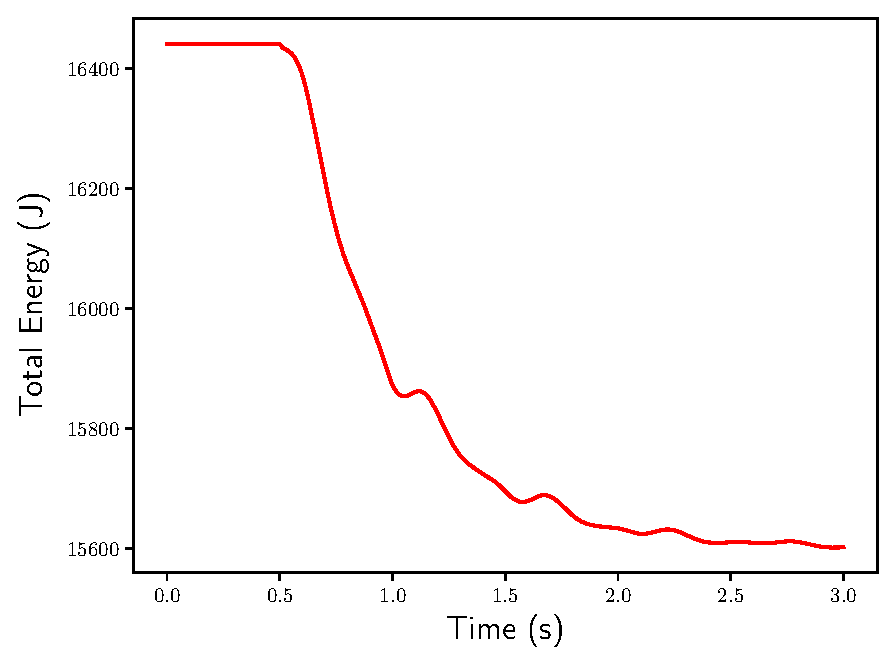
\includegraphics[width=0.48\linewidth]{TwoDimension/Hamiltonian.eps}%
		\label{fig:Ham}}
	\subfloat[Lyapunov function]{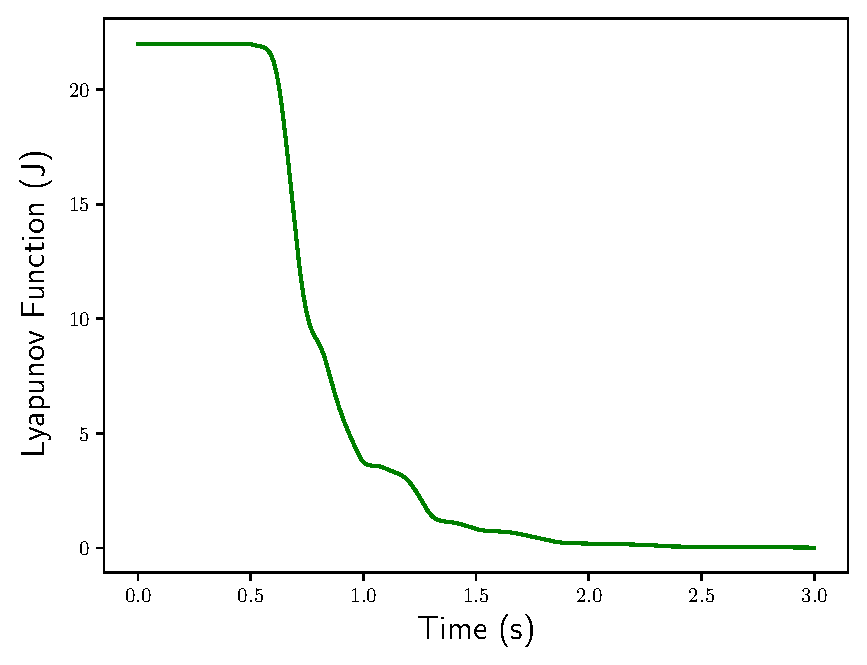
\includegraphics[width=0.48\linewidth]{TwoDimension/Lyapunov.eps}%
		\label{fig:Lyap}}
	\caption{Total energy and Lyapunov Function}
	\label{fig:HL2D}
\end{figure}
}

}



\section{Conclusions and further work}


\frame{\frametitle{Conclusions and further work}
Results:
\begin{itemize}
  \item Obtained a 2D polar representation of 2D SWE using port-Hamiltonian equations;
  \item Obtained a 1D reduced model assuming revolution symmetry;
  \item Approximated the {\color{red}{nonlinear} }equations using a power-preserving method;
  \item Nonlinear time-domain simulations were performed;
  \item A simple output feedback controller was tested in simulations.
\end{itemize}
\pause
Further work:
\begin{itemize}
  \item Couple with actuator dynamics;
  \item Use other feedback control strategies (control by interconnection, impledance control);
  \item How to deal with shocks?
\end{itemize}
}



% \frame{\frametitle{A few references:}
% \scriptsize
	  % \begin{thebibliography}{10}    
		  % \beamertemplatearticlebibitems
		  % \bibitem{Golo2004}
			% Golo, G., Talasila, V., Van Der Schaft, A., and Maschke.
			% \newblock Hamiltonian discretization of boundary control systems.
			% \newblock {\em Automatica}, 2004.
		  % \bibitem{Moulla2012}
			% Moulla, R., Lefevre, L., and Maschke.,B
			% \newblock Pseudo-spectral methods for the spatial symplectic reduction of open systems of conservation laws.
			% \newblock {\em Journal of Computational Physics}, 2012.	
		  % \bibitem{Voss}
			% Voss, T. and Scherpen, J.
			% \newblock Structure preserving spatial discretization of a 1-D piezoelectric Timoshenko beam.
			% \newblock {\em Multiscale Modeling and Simulation}, 2011.	
		  % \bibitem{LeGorrec}
			% Le Gorrec, Y., Zwart , H. and Maschke, B.
			% \newblock Dirac structures and boundary control systems associated with skew-symmetric differential operators.
			% \newblock {\em SIAM Journal of Control and Optimization}, 2005.	
  		  % \bibitem{Morris}
			% Morris, K. and Ozer, A.
			% \newblock Strong stabilization of piezoelectric beams with magnetic effects.
			% \newblock {\em 5nd IEEE Conference on Decision and Control}, 2013.	
		  % \beamertemplatebookbibitems
		  % \bibitem{BANKS1996}
			% Banks, H., Smith, R., and Wang, Y.
			% \newblock Smart Material Structures.
			% \newblock Wiley, 1996.

  % \end{thebibliography}

% }
\frame{\frametitle{}


	\vspace{2cm}
	\begin{flushright}
		\Large
		 Thank you for your attention!
	\end{flushright}
	
	
	% \vspace{2cm}
	% \small
	% More results, codes, etc.:
	% \url{http://github.com/flavioluiz/port-hamiltonian}
	% \url{http://flavioluiz.github.io}
	
}


\end{document}
